%% NOTAS


%poner disclaimer de que no se puede utilizar este apunte para diseño. Para diseño, se debe referir a la ultima version del codigo.

%Apunte interno de FIUBA, cn la finalidad de realizar una introduccion.

%Poner como esta estructurado el codigo.

% Poner la version que usamos.

% Poner foto de caldera (extracto de plano gonella), poner las valvulas de seguridad, mostrar pid, mostrar foto de adentro de domo, mostrar firetube boiler con las dos PSV.

% Espesor, derivacion, ver si pongo algo de las tapas, ver si pongo algo de los stays, poner cuanto puedo agujerear el domo.

% Mostrar límite de jurisdicción del código.

%\section{Introducción}

%Poner los nombres en inglés, poner qué es ASME. Poner el disclaimer.

%ver las tolerancias de fabricación.

% Estampa, código de diseño y fabricación.

%ajustar el ejemplo 1145.

%embeberle los archivos EES que haya usado.
%\mirar los companions

%dividir mejor en secciones el codigo

%buscar los calculos que netrego VPI de sus tachos, a ver como presentan

%ver si pongo los formularios que me desargue



%##########################################

\section{Introducción}

\subsection{alcance del código}
Acá hablar de la esctructura

Poner qué es y qué no es el código.

Cómo interactúa con un mercado, con un arbitraje, que es diseño y fabricación, estampas parciales y completas.

La diferencia con hacer un hermoso cálculo con la teoría de las cáscaras o con los elementos finitos, pero hay partes que después quedan descubiertas. El código es integral.

Código es como empírico, ojo con los márgenes que toma, ASME lo cambia, y los americanos son conocidos por sobredimensionar. Los europeos lo hicieron mejor y tuvieron que achicar el margen de seguridad.

\subsection{calderas acuotubular y pirotubular}
Mostrar caldera paquete, fotos, mostrar fotos internas de domos


\begin{figure}[ht]
    \centerline{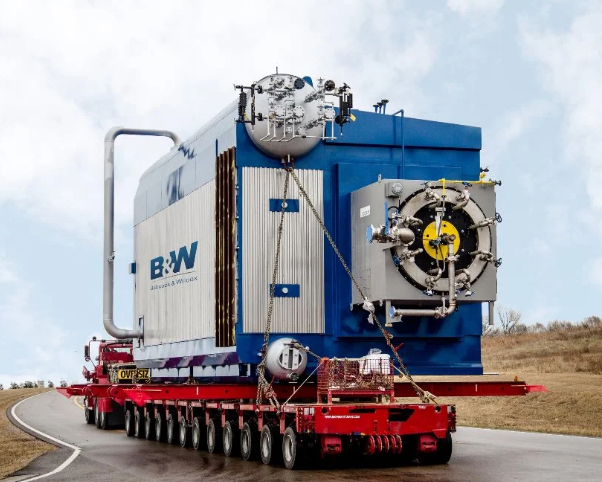
\includegraphics[scale=0.6]{b_w_boiler_01.png}}
    \caption{\textit{TBD.}}
    \label{im:b_w_boiler_01}
\end{figure}

\begin{figure}[ht]
    \centerline{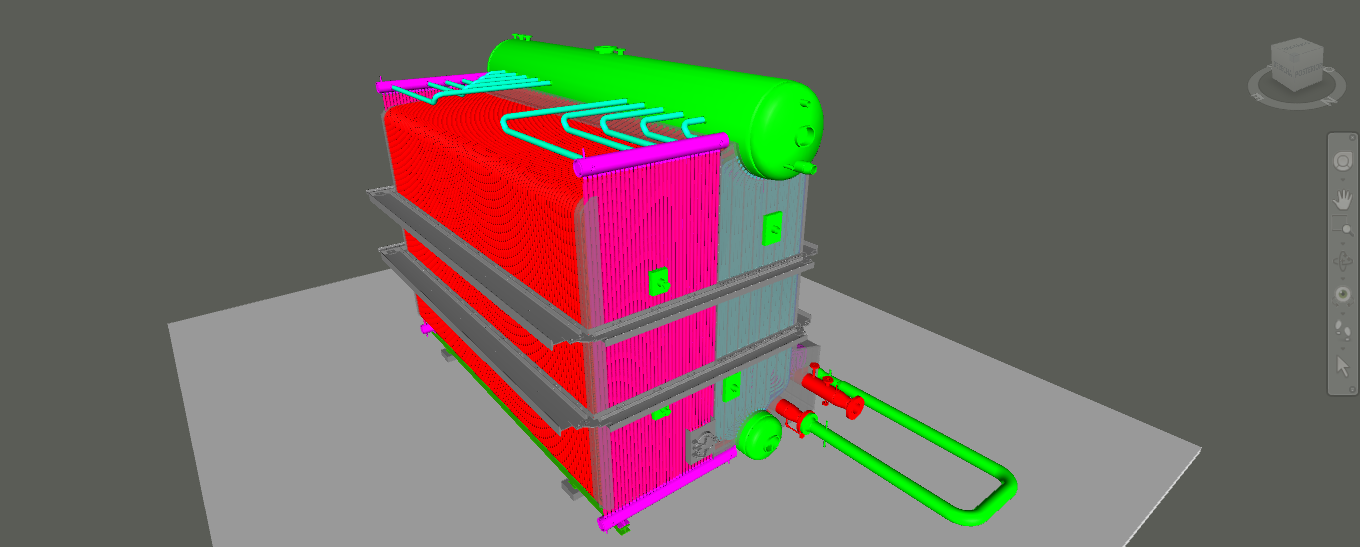
\includegraphics[scale=0.2]{b_w_boiler_02.png}}
    \caption{\textit{TBD.}}
    \label{im:b_w_boiler_02}
\end{figure}

\begin{figure}[ht]
    \centerline{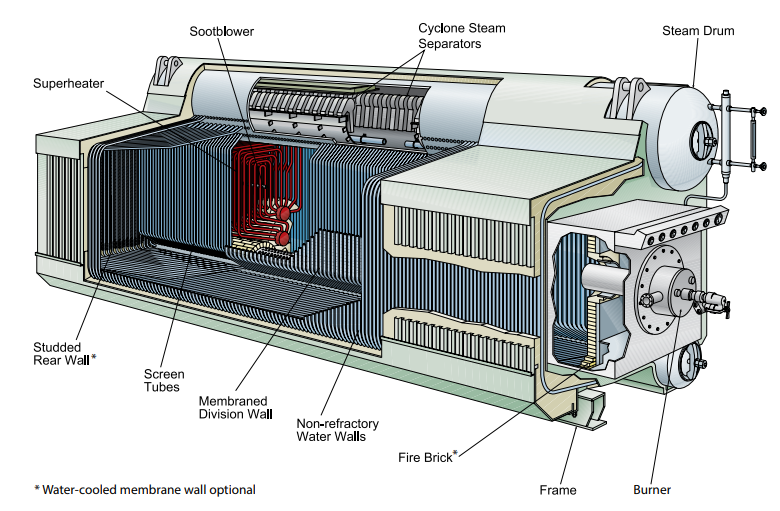
\includegraphics[scale=0.6]{b_w_boiler_03.png}}
    \caption{\textit{TBD.}}
    \label{im:b_w_boiler_03}
\end{figure}


\begin{figure}[ht]
    \centerline{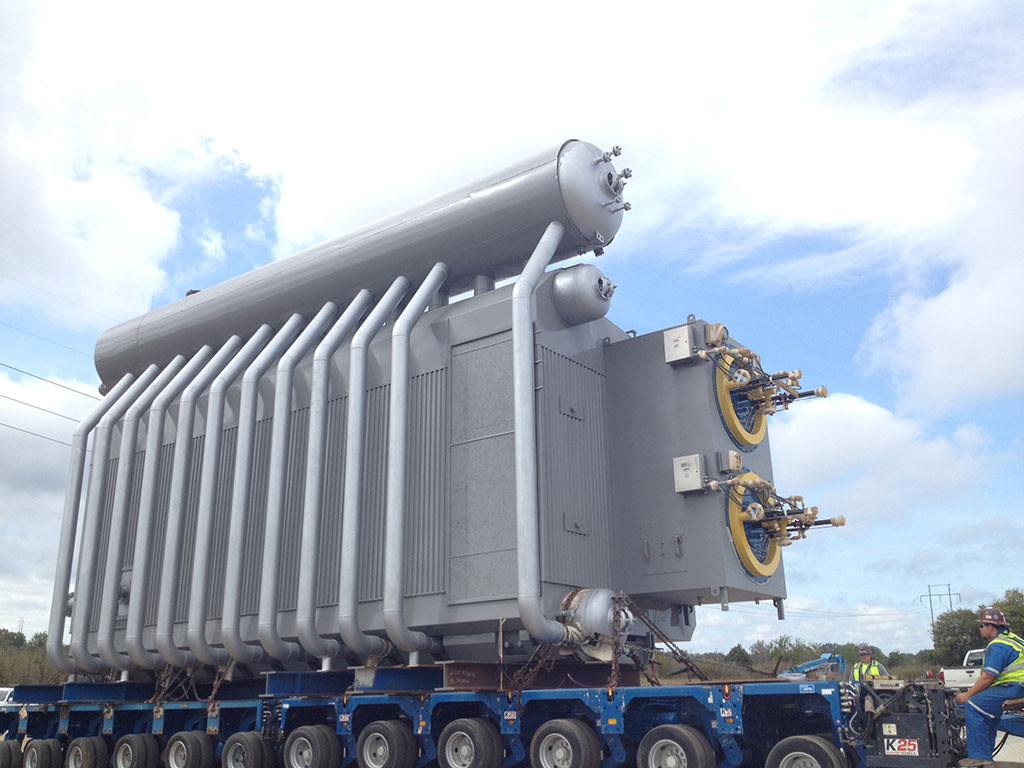
\includegraphics[scale=0.4]{b_w_boiler_04.jpg}}
    \caption{\textit{TBD.}}
    \label{im:b_w_boiler_04}
\end{figure}

\begin{figure}[ht]
    \centerline{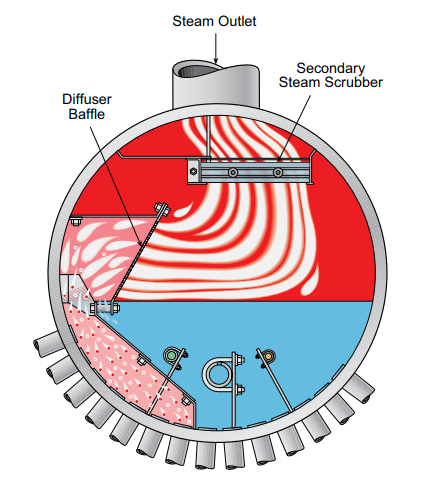
\includegraphics[scale=0.6]{drum_internals_01.png}}
    \caption{\textit{TBD.}}
    \label{im:drum_internals_01}
\end{figure}

\begin{figure}[ht]
    \centerline{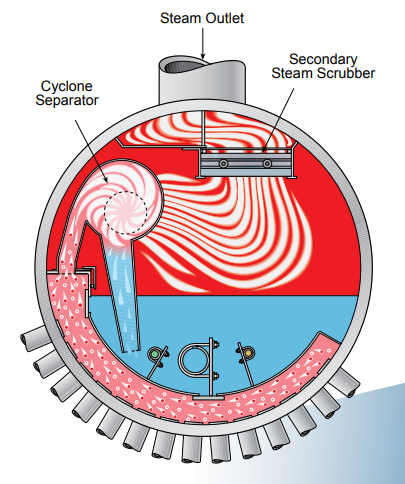
\includegraphics[scale=0.6]{drum_internals_02.png}}
    \caption{\textit{TBD.}}
    \label{im:drum_internals_02}
\end{figure}

\begin{figure}[ht]
    \centerline{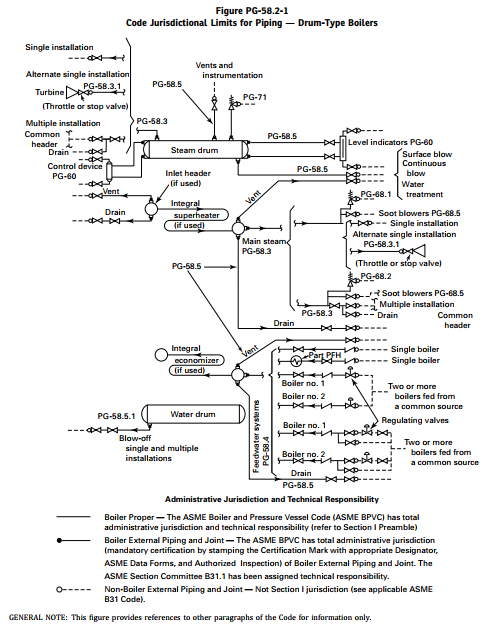
\includegraphics[scale=0.6]{PG-58.2-1.png}}
    \caption{\textit{Límite de la jurisdicción del BPVC para las cañerías. Para calderas con domo.}}
    \label{im:PG-58.2-1}
\end{figure}


% https://www.youtube.com/watch?v=Hi8GlGR7-tA
% http://hdboilerparts.com/1-boiler-steam-drum.html
% imagen de los planos de agrest
% sacar imagenes de estos videos
% ver los ajustes de las figuras y tablas
% ir armando datos para los TPs. Armarme un excel, y resolverlos todos.
% Ver si con python puedo hacer una mejor interpolacion para esos datos que hice con EES lineal.


\subsection{limites de jurisdiccion}
diferenciar con codigo ASME B31.1